\documentclass[11pt,a4paper]{report}
\usepackage[textwidth=37em,vmargin=30mm]{geometry}
\usepackage{calc,xunicode,amsmath,amssymb,paralist,enumitem,tabu,booktabs,datetime2,xeCJK,xeCJKfntef,listings}
\usepackage{tocloft,fancyhdr,tcolorbox,xcolor,graphicx,eso-pic,xltxtra,xelatexemoji}

\newcommand{\envyear}[0]{2025}
\newcommand{\envdatestr}[0]{2025-08-15}
\newcommand{\envfinaldir}[0]{webdb/2025/20250815/final}

\usepackage[hidelinks]{hyperref}
\hypersetup{
    colorlinks=false,
    pdfpagemode=FullScreen,
    pdftitle={Web Digest - \envdatestr}
}

\setlength{\cftbeforechapskip}{10pt}
\renewcommand{\cftchapfont}{\rmfamily\bfseries\large\raggedright}
\setlength{\cftbeforesecskip}{2pt}
\renewcommand{\cftsecfont}{\sffamily\small\raggedright}

\setdefaultleftmargin{2em}{2em}{1em}{1em}{1em}{1em}

\usepackage{xeCJK,xeCJKfntef}
\xeCJKsetup{PunctStyle=plain,RubberPunctSkip=false,CJKglue=\strut\hskip 0pt plus 0.1em minus 0.05em,CJKecglue=\strut\hskip 0.22em plus 0.2em}
\XeTeXlinebreaklocale "zh"
\XeTeXlinebreakskip = 0pt


\setmainfont{Brygada 1918}
\setromanfont{Brygada 1918}
\setsansfont{IBM Plex Sans}
\setmonofont{JetBrains Mono NL}
\setCJKmainfont{Noto Serif CJK SC}
\setCJKromanfont{Noto Serif CJK SC}
\setCJKsansfont{Noto Sans CJK SC}
\setCJKmonofont{Noto Sans CJK SC}

\setlength{\parindent}{0pt}
\setlength{\parskip}{8pt}
\linespread{1.15}

\lstset{
	basicstyle=\ttfamily\footnotesize,
	numbersep=5pt,
	backgroundcolor=\color{black!5},
	showspaces=false,
	showstringspaces=false,
	showtabs=false,
	tabsize=2,
	captionpos=b,
	breaklines=true,
	breakatwhitespace=true,
	breakautoindent=true,
	linewidth=\textwidth
}






\newcommand{\coverpic}[2]{
    % argv: itemurl, authorname
    Cover photo by #2~~(\href{#1}{#1})
}
\newcommand{\makeheader}[0]{
    \begin{titlepage}
        % \newgeometry{hmargin=15mm,tmargin=21mm,bmargin=12mm}
        \begin{center}
            
            \rmfamily\scshape
            \fontspec{BaskervilleF}
            \fontspec{Old Standard}
            \fontsize{59pt}{70pt}\selectfont
            WEB\hfill DIGEST
            
            \vfill
            % \vskip 30pt
            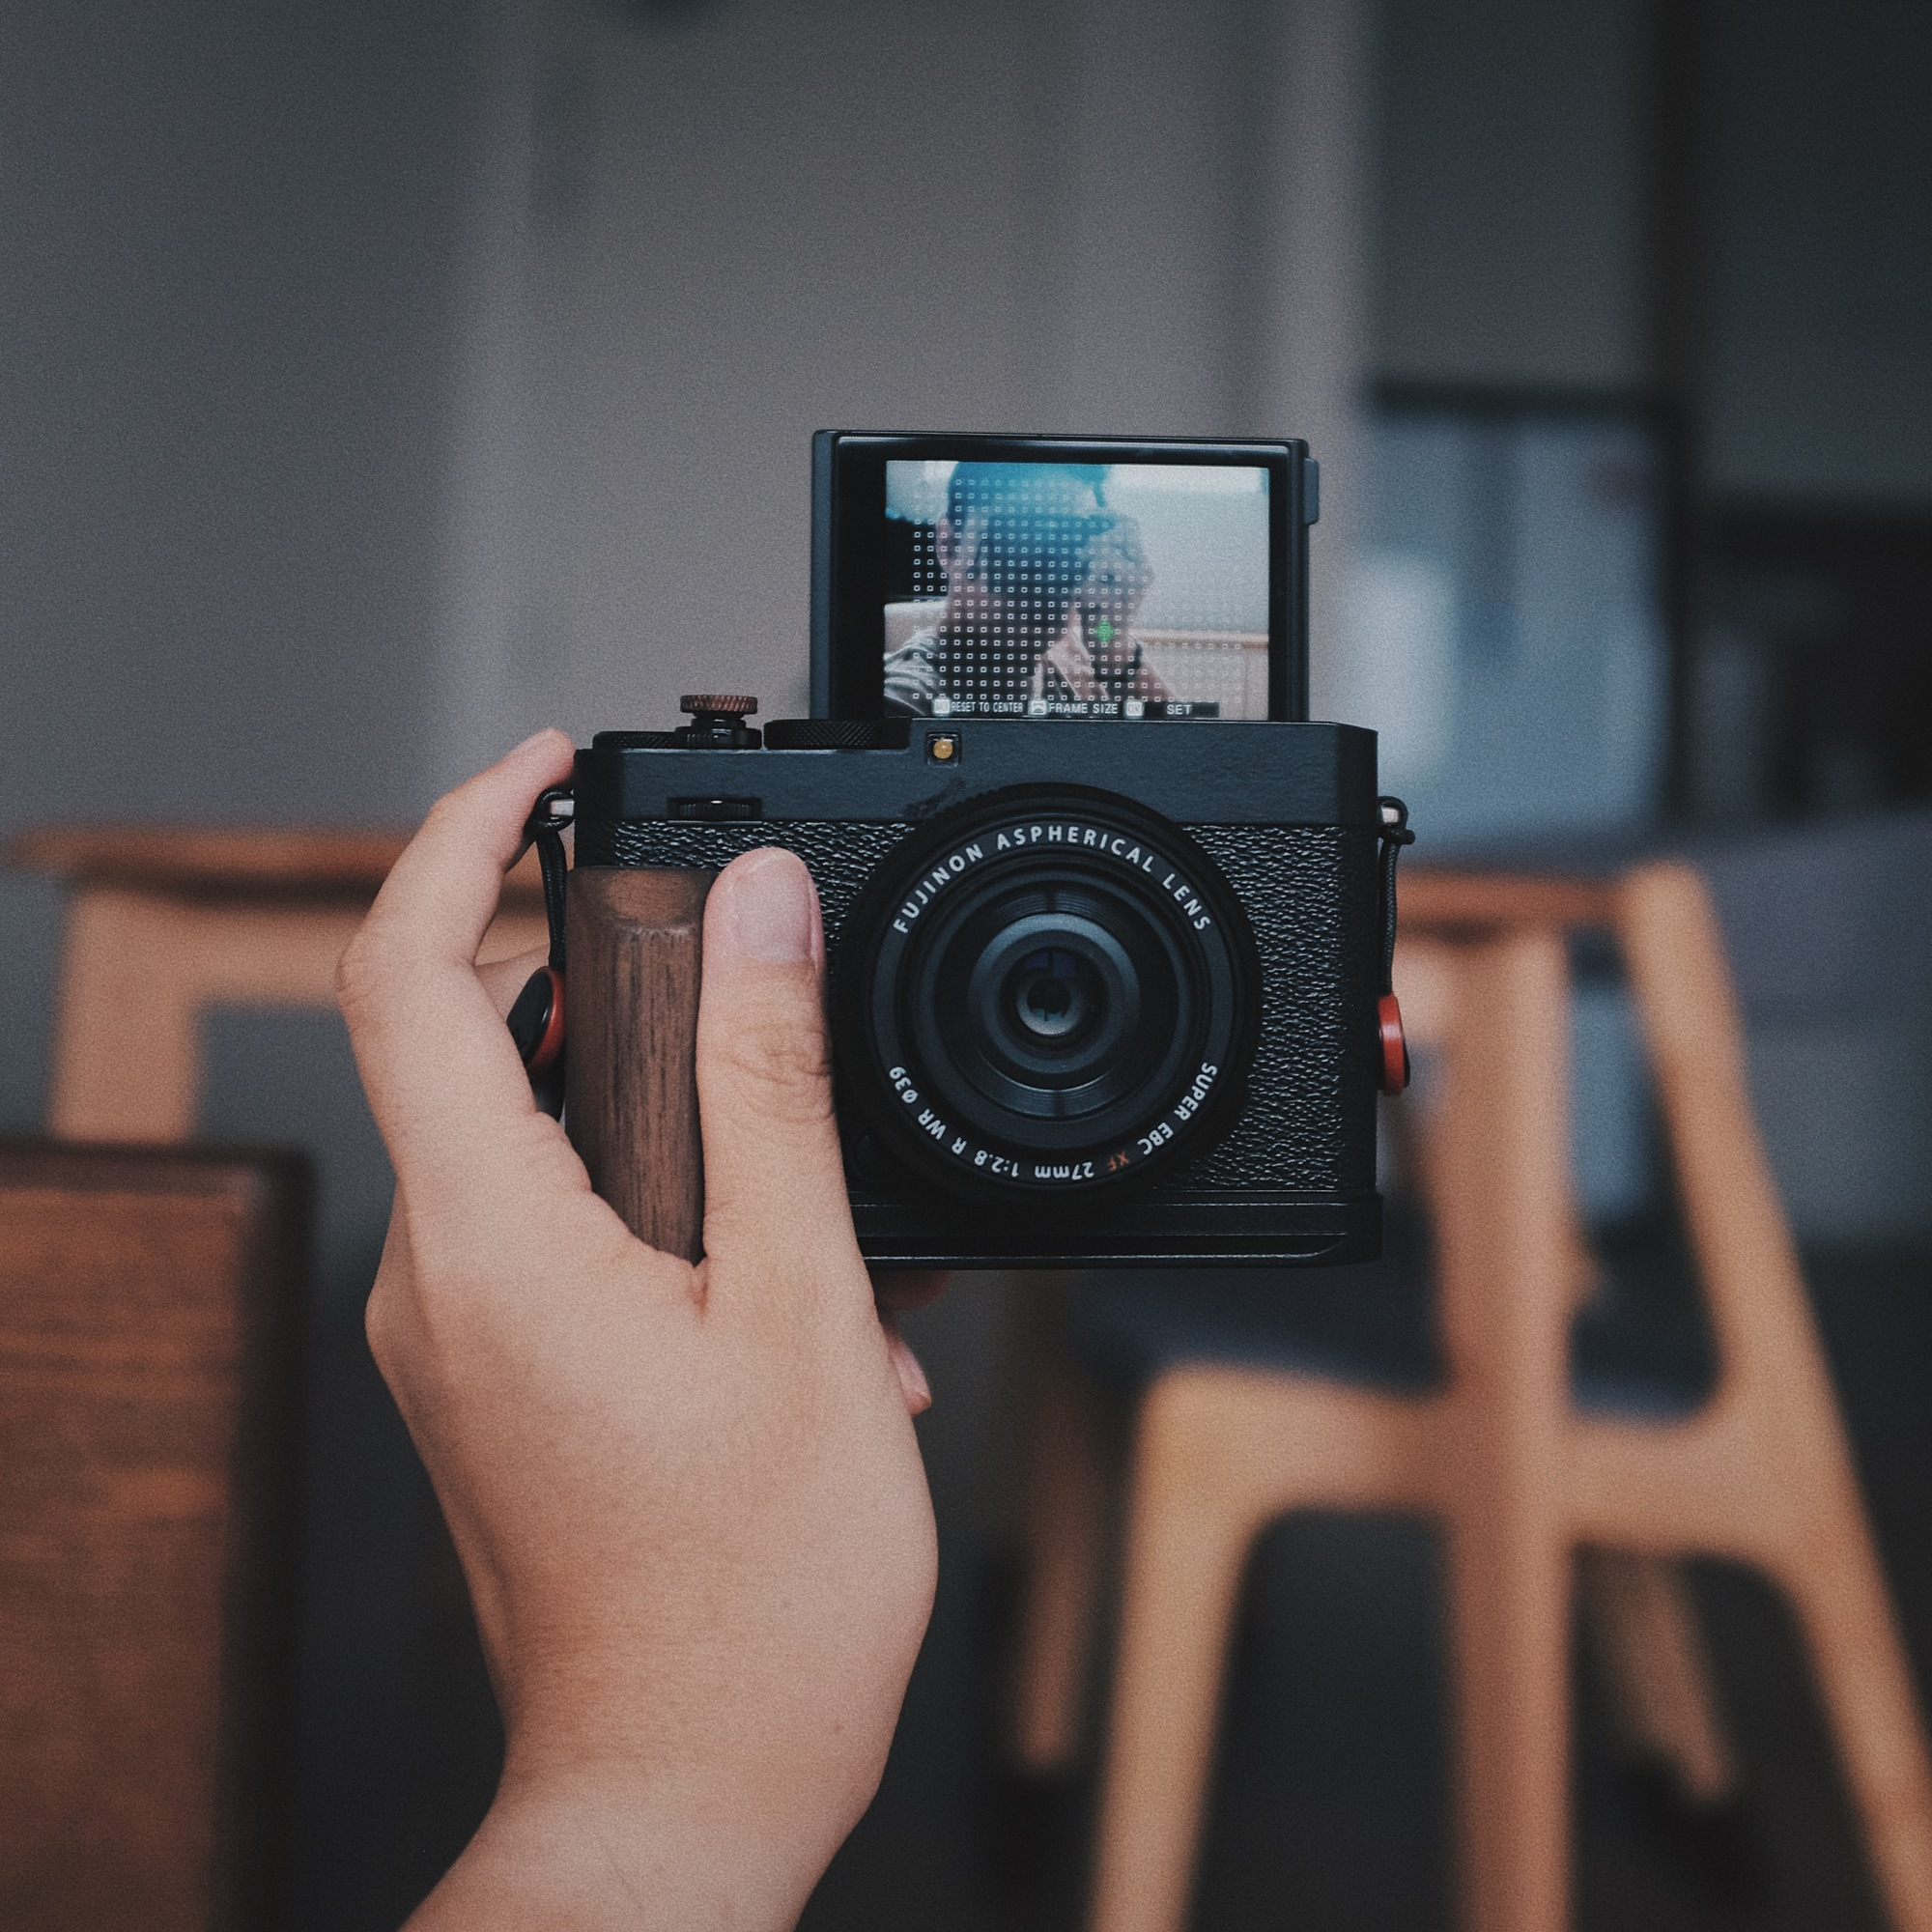
\includegraphics[width=\linewidth]{\envfinaldir/coverpic-prod.jpg}\par
            % \vskip 30pt
            \vfill

            \normalsize\rmfamily\scshape
            \copyright{} The Web Digest Project \hfill\large \envdatestr
        \end{center}
    \end{titlepage}
    % \restoregeometry
}
\newcommand{\simplehref}[1]{%
    \textcolor{blue!80!green}{\href{#1}{#1}}%
}
\renewcommand{\contentsname}{\center\Huge\sffamily\bfseries Contents\par\vskip 20pt}
\newcounter{ipartcounter}
\setcounter{ipartcounter}{0}
\newcommand{\ipart}[1]{
    % \vskip 20pt
    \clearpage
    \stepcounter{ipartcounter}
    \phantomsection
    \addcontentsline{toc}{chapter}{#1}
    % \begin{center}
    %     \Huge
    %     \sffamily\bfseries
    %     #1
    % \end{center}
    % \vskip 20pt plus 7pt
}
\newcounter{ichaptercounter}
\setcounter{ichaptercounter}{0}
\newcommand{\ichapter}[1]{
    % \vskip 20pt
    \clearpage
    \stepcounter{ichaptercounter}
    \phantomsection
    \addcontentsline{toc}{section}{\numberline{\arabic{ichaptercounter}}#1}
    \begin{center}
        \Huge
        \sffamily\bfseries
        #1
    \end{center}
    \vskip 20pt plus 7pt
}
\newcommand{\entrytitlefont}[1]{\subsection*{\raggedright\Large\sffamily\bfseries#1}}
\newcommand{\entryitemGeneric}[2]{
    % argv: title, url
    \parbox{\linewidth}{
        \entrytitlefont{#1}\par\vskip 5pt
        \footnotesize\ttfamily\mdseries
        \simplehref{#2}
    }\vskip 11pt plus 11pt minus 1pt
}
\newcommand{\entryitemGithub}[3]{
    % argv: title, url, desc
    \parbox{\linewidth}{
        \entrytitlefont{#1}\par\vskip 5pt
        \footnotesize\ttfamily\mdseries
        \simplehref{#2}\par\vskip 5pt
        \small\rmfamily\mdseries#3
    }\vskip 11pt plus 11pt minus 1pt
}
\newcommand{\entryitemAp}[3]{
    % argv: title, url, desc
    \parbox{\linewidth}{
        \entrytitlefont{#1}\par\vskip 5pt
        \footnotesize\ttfamily\mdseries
        \simplehref{#2}\par\vskip 5pt
        \small\rmfamily\mdseries#3
    }\vskip 11pt plus 11pt minus 1pt
}
\newcommand{\entryitemHackernews}[3]{
    % argv: title, hnurl, rawurl
    % \parbox{\linewidth}{
    %     \entrytitlefont{#1}\par\vskip 5pt
    %     \footnotesize\ttfamily\mdseries
    %     \simplehref{#3}\par
    %     \textcolor{black!50}{\href{#2}{#2}}
    % }\vskip 11pt plus 11pt minus 1pt
    \begin{minipage}{\linewidth}
            \entrytitlefont{#1}\par\vskip 5pt
            \footnotesize\ttfamily\mdseries
            \simplehref{#3}\par
            \textcolor{black!50}{\href{#2}{#2}}
    \end{minipage}\par\vskip 11pt plus 11pt minus 1pt
}







\begin{document}

\makeheader

\tableofcontents\clearpage




\ipart{Developers}
\ichapter{Hacker News}
\entryitemTwoLinks{Steve Wozniak: Life to me was never about accomplishment, but about happiness}{https://news.ycombinator.com/item?id=44903803}{https://yro.slashdot.org/comments.pl?sid=23765914\&cid=65583466}

\entryitemTwoLinks{"Privacy preserving age verification" is bullshit}{https://news.ycombinator.com/item?id=44903351}{https://pluralistic.net/2025/08/14/bellovin/}

\entryitemTwoLinks{Streaming services are driving viewers back to piracy}{https://news.ycombinator.com/item?id=44902797}{https://www.theguardian.com/film/2025/aug/14/cant-pay-wont-pay-impoverished-streaming-services-are-driving-viewers-back-to-piracy}

\entryitemTwoLinks{Gemma 3 270M: Compact model for hyper-efficient AI}{https://news.ycombinator.com/item?id=44902148}{https://developers.googleblog.com/en/introducing-gemma-3-270m/}

\entryitemTwoLinks{I made a real-time C/C++/Rust build visualizer}{https://news.ycombinator.com/item?id=44902127}{https://danielchasehooper.com/posts/syscall-build-snooping/}

\entryitemTwoLinks{Show HN: I built a free alternative to Adobe Acrobat PDF viewer}{https://news.ycombinator.com/item?id=44901683}{https://github.com/embedpdf/embed-pdf-viewer}

\entryitemTwoLinks{Kodak has no plans to cease, go out of business, or file for bankruptcy}{https://news.ycombinator.com/item?id=44901330}{https://www.kodak.com/en/company/blog-post/statement-regarding-misleading-media-reports/}

\entryitemTwoLinks{Meta's flirty AI chatbot invited a retiree to New York}{https://news.ycombinator.com/item?id=44901123}{https://www.reuters.com/investigates/special-report/meta-ai-chatbot-death/}

\entryitemTwoLinks{Jujutsu and Radicle}{https://news.ycombinator.com/item?id=44900455}{https://radicle.xyz/2025/08/14/jujutsu-with-radicle}

\entryitemTwoLinks{Is chain-of-thought AI reasoning a mirage?}{https://news.ycombinator.com/item?id=44900340}{https://www.seangoedecke.com/real-reasoning/}

\entryitemTwoLinks{"None of These Books Are Obscene": Judge Strikes Down Much of FL's Book Ban Bill}{https://news.ycombinator.com/item?id=44900302}{https://bookriot.com/penguin-random-house-florida-lawsuit/}

\entryitemTwoLinks{Why LLMs can't really build software}{https://news.ycombinator.com/item?id=44900116}{https://zed.dev/blog/why-llms-cant-build-software}

\entryitemTwoLinks{Blood oxygen monitoring returning to Apple Watch in the US}{https://news.ycombinator.com/item?id=44899999}{https://www.apple.com/newsroom/2025/08/an-update-on-blood-oxygen-for-apple-watch-in-the-us/}

\entryitemTwoLinks{NSF and Nvidia award Ai2 \$152M to support building an open AI ecosystem}{https://news.ycombinator.com/item?id=44899935}{https://allenai.org/blog/nsf-nvidia}

\entryitemTwoLinks{US Wholesale Inflation Rises by Most in 3 Years}{https://news.ycombinator.com/item?id=44899685}{https://www.bloomberg.com/news/articles/2025-08-14/us-producer-prices-rise-by-most-in-three-years-on-services}

\entryitemTwoLinks{Wholesale prices rose 0.9\% in July, more than expected}{https://news.ycombinator.com/item?id=44899639}{https://www.cnbc.com/2025/08/14/ppi-inflation-report-july-2025-.html}

\entryitemTwoLinks{Linux address space isolation revived after lowering performance hit}{https://news.ycombinator.com/item?id=44899488}{https://www.phoronix.com/news/Linux-ASI-Lower-Overhead}

\entryitemTwoLinks{How to rig elections [video]}{https://news.ycombinator.com/item?id=44899415}{https://media.ccc.de/v/why2025-218-how-to-rig-elections}

\entryitemTwoLinks{New protein therapy shows promise as antidote for carbon monoxide poisoning}{https://news.ycombinator.com/item?id=44899339}{https://www.medschool.umaryland.edu/news/2025/new-protein-therapy-shows-promise-as-first-ever-antidote-for-carbon-monoxide-poisoning.html}

\entryitemTwoLinks{Org-social is a decentralized social network that runs on Org Mode}{https://news.ycombinator.com/item?id=44898955}{https://github.com/tanrax/org-social}\ichapter{Phoronix}
\entryitemGeneric{\hskip 0pt{}TrueNAS 25.10 Begins Testing With Faster Performance, 400GbE Networking}{https://www.phoronix.com/news/TrueNAS-25.10-Testing}

\entryitemGeneric{\hskip 0pt{}Valkey 9.0-rc1 Taps AVX-512 For String-To-Integer Conversion For ~19\% Gain}{https://www.phoronix.com/news/Valkey-9.0-rc1-Released}

\entryitemGeneric{\hskip 0pt{}Ubuntu 25.10 Continues Preparing For RISC-V RVA23 Baseline Requirement}{https://www.phoronix.com/news/RISC-V-RVA23-Progress-Ubuntu}

\entryitemGeneric{\hskip 0pt{}VirtualBox 7.2 Released With Windows 11 ARM Support, Linux 6.16 Compatibility}{https://www.phoronix.com/news/VirtualBox-7.2-Released}

\entryitemGeneric{\hskip 0pt{}AMD Ryzen Threadripper PRO 9995WX Performance With TRX50 + Quad Channel DDR5}{https://www.phoronix.com/review/amd-threadripper-9995wx-trx50}

\entryitemGeneric{\hskip 0pt{}Intel's Habana Labs / Gaudi Accelerator Driver Maintainer Is Leaving The Company}{https://www.phoronix.com/news/Gaudi-2025-Maintainer-Leaving}

\entryitemGeneric{\hskip 0pt{}KDE Gear 25.08 Released With Improvements For Many KDE Apps}{https://www.phoronix.com/news/KDE-Gear-25.08}

\entryitemGeneric{\hskip 0pt{}AMDXDNA Improvements \& New Rockchip NPU Accelerator Driver For Linux 6.18}{https://www.phoronix.com/news/DRM-Misc-Next-Linux-6.18}

\entryitemGeneric{\hskip 0pt{}LibreOffice 26.2 To Better Handle Documents With Restricted Embedded Fonts}{https://www.phoronix.com/news/LibreOffice-Restricted-Fonts}


\ipart{Developers~~~~(zh-Hans)}
\ichapter{Solidot}
\entryitemGeneric{\hskip 0pt{}研究认为社交媒体的问题无法得到修正}{https://www.solidot.org/story?sid=82047}

\entryitemGeneric{\hskip 0pt{}挪威指责俄黑客破坏其水坝}{https://www.solidot.org/story?sid=82046}

\entryitemGeneric{\hskip 0pt{}韩国星巴克要求顾客不要将打印机和台式机带到店里}{https://www.solidot.org/story?sid=82045}

\entryitemGeneric{\hskip 0pt{}猫的痴呆症与人类相似}{https://www.solidot.org/story?sid=82044}

\entryitemGeneric{\hskip 0pt{}地震的长尾效应}{https://www.solidot.org/story?sid=82043}

\entryitemGeneric{\hskip 0pt{}美国 在 AI 芯片货物中装定位追踪器}{https://www.solidot.org/story?sid=82042}

\entryitemGeneric{\hskip 0pt{}身份证关联疾病信息}{https://www.solidot.org/story?sid=82041}

\entryitemGeneric{\hskip 0pt{}步行友好的城市增加居民的步行次数}{https://www.solidot.org/story?sid=82040}

\entryitemGeneric{\hskip 0pt{}马斯克威胁苹果,想要提高其 AI 应用 Grok 的排名}{https://www.solidot.org/story?sid=82039}

\entryitemGeneric{\hskip 0pt{}Google 允许美国印度用户选择他们喜欢的内容来源}{https://www.solidot.org/story?sid=82038}

\entryitemGeneric{\hskip 0pt{}《K-POP:猎魔女团》成为 Netflix 史上观看次数最多的动漫电影}{https://www.solidot.org/story?sid=82037}

\entryitemGeneric{\hskip 0pt{}你一生中被小行星砸到的概率}{https://www.solidot.org/story?sid=82036}

\entryitemGeneric{\hskip 0pt{}性逆转在鸟类中间很常见}{https://www.solidot.org/story?sid=82035}

\entryitemGeneric{\hskip 0pt{}英国政府建议居民删除邮件以节省用水}{https://www.solidot.org/story?sid=82034}

\entryitemGeneric{\hskip 0pt{}Threads 月活跃用户数突破 4 亿}{https://www.solidot.org/story?sid=82033}

\entryitemGeneric{\hskip 0pt{}Do Kwon 对欺诈指控认罪}{https://www.solidot.org/story?sid=82032}

\entryitemGeneric{\hskip 0pt{}Perplexity 报价 345 亿美元收购 Chrome}{https://www.solidot.org/story?sid=82031}

\entryitemGeneric{\hskip 0pt{}Debian GNU/Hurd 2025 释出}{https://www.solidot.org/story?sid=82030}

\entryitemGeneric{\hskip 0pt{}亚马逊宽带卫星在轨数量突破 100 颗}{https://www.solidot.org/story?sid=82029}

\entryitemGeneric{\hskip 0pt{}有 133 亿年历史的最古老黑洞}{https://www.solidot.org/story?sid=82028}\ichapter{V2EX}
\entryitemGeneric{\hskip 0pt{}[C++] 记录一次踩坑过程(clion + cmake + vcpkg)}{https://www.v2ex.com/t/1152503}

\entryitemGeneric{\hskip 0pt{}[macOS] mac 更了公测 3 啥也没干一直在吃内存吃了几十个 g 了}{https://www.v2ex.com/t/1152502}

\entryitemGeneric{\hskip 0pt{}[程序员] 关于在 Java 里面实现命名参数的一些想法}{https://www.v2ex.com/t/1152501}

\entryitemGeneric{\hskip 0pt{}[Solana] 换 V2EX 币的时候提示 okx 这个主网币不足怎么解决?}{https://www.v2ex.com/t/1152500}

\entryitemGeneric{\hskip 0pt{}[Bitcoin] 比特币相关代码,技术!}{https://www.v2ex.com/t/1152499}

\entryitemGeneric{\hskip 0pt{}[问与答] 最近听周边人都在人心惶惶的谈论:房东税;大家如何看待此问题?真的是穷疯了?}{https://www.v2ex.com/t/1152498}

\entryitemGeneric{\hskip 0pt{}[职场话题] 白天上班,晚上拼副业,真的很累}{https://www.v2ex.com/t/1152497}

\entryitemGeneric{\hskip 0pt{}[推广] 最近 cusor 封掉以后切 IDE, claude code 体验效果还不错,有需要可以免费试试}{https://www.v2ex.com/t/1152496}

\entryitemGeneric{\hskip 0pt{}[加密货币] 关于加密货币,我是很多年的玩家了,有感而分享,希望看到的人少走弯路,节省点学费}{https://www.v2ex.com/t/1152495}

\entryitemGeneric{\hskip 0pt{}[英雄联盟] 英雄联盟腾讯为什么要用机器人恶心玩家?}{https://www.v2ex.com/t/1152494}

\entryitemGeneric{\hskip 0pt{}[分享创造] [求拍砖] 爆肝 3 个多月,为 AI 应用商业化造了个 ``聚合服务'',大家觉得有需求吗?}{https://www.v2ex.com/t/1152493}

\entryitemGeneric{\hskip 0pt{}[Windows] Windows 11 24H2 的输入法小改进}{https://www.v2ex.com/t/1152490}

\entryitemGeneric{\hskip 0pt{}[投资] 赚认知的钱,我为什么会买一个点仓位的 V 币}{https://www.v2ex.com/t/1152489}

\entryitemGeneric{\hskip 0pt{}[分享创造] 搞了个 n8n 中文工作流分享站 n8ncn.io,求大佬们拍砖}{https://www.v2ex.com/t/1152488}

\entryitemGeneric{\hskip 0pt{}[Linux] 有新闻说 Ubuntu 的下一个服务器版本,也就是 Ubuntu Server 25.10,默认不再提供 wget 命令}{https://www.v2ex.com/t/1152483}

\entryitemGeneric{\hskip 0pt{}[分享发现] 学习百词斩助手插件,并且升级改造}{https://www.v2ex.com/t/1152482}

\entryitemGeneric{\hskip 0pt{}[VXNA] 申请收录 https://www.xwenming.com,之前有个别帖子涉及了不好的内容,已删除}{https://www.v2ex.com/t/1152480}

\entryitemGeneric{\hskip 0pt{}[职场话题] 走出浪浪山,小妖怪也能卷进大厂了}{https://www.v2ex.com/t/1152478}

\entryitemGeneric{\hskip 0pt{}[生活] 很久没管的 wx 小程序被投诉了}{https://www.v2ex.com/t/1152475}

\entryitemGeneric{\hskip 0pt{}[问与答] 有小功率的桌面音响推荐吗}{https://www.v2ex.com/t/1152474}

\entryitemGeneric{\hskip 0pt{}[Linux] 求可以装在 U 盘的不可变 Linux 发行版}{https://www.v2ex.com/t/1152472}

\entryitemGeneric{\hskip 0pt{}[Solana] \$V2EX,拿住就好!}{https://www.v2ex.com/t/1152471}

\entryitemGeneric{\hskip 0pt{}[Solana] 有人愿意交易一点点 solana 的 sol 币么?}{https://www.v2ex.com/t/1152469}

\entryitemGeneric{\hskip 0pt{}[互联网] 猛然发现自己订阅了国内外几乎主要的网盘}{https://www.v2ex.com/t/1152468}

\entryitemGeneric{\hskip 0pt{}[问与答] 真正开始做一件事的时候很难}{https://www.v2ex.com/t/1152466}

\entryitemGeneric{\hskip 0pt{}[职场话题] 到底是继续干程序员还是能干什么其他的 对未来有点迷茫}{https://www.v2ex.com/t/1152465}

\entryitemGeneric{\hskip 0pt{}[Apple] Mac 能像 Windows 一样通过触控板快速切换程序吗?}{https://www.v2ex.com/t/1152464}

\entryitemGeneric{\hskip 0pt{}[问与答] 请问一个关于 sing-box 的 dns 规则分流问题}{https://www.v2ex.com/t/1152463}

\entryitemGeneric{\hskip 0pt{}[Solana] 再次 0.013 了!有上车的吗!}{https://www.v2ex.com/t/1152462}

\entryitemGeneric{\hskip 0pt{}[分享创造] Seele AI - 最近超火的 3D Game 生成器}{https://www.v2ex.com/t/1152461}

\entryitemGeneric{\hskip 0pt{}[问与答] 逐渐对家人失望了,是我太幼稚不成熟的表现吗?}{https://www.v2ex.com/t/1152460}

\entryitemGeneric{\hskip 0pt{}[Apple] macOS 动态壁纸 是个坑?}{https://www.v2ex.com/t/1152458}

\entryitemGeneric{\hskip 0pt{}[macOS] Apple Books,库克的圈套}{https://www.v2ex.com/t/1152457}

\entryitemGeneric{\hskip 0pt{}[Solana] Leger 的 Solana 应用签名报错 0x6a81 有没有 C 语言大佬给他们修修}{https://www.v2ex.com/t/1152455}

\entryitemGeneric{\hskip 0pt{}[分享创造] 用 Claude Code 和 v0 写了一个基于 Ollama 的本地 RAG 的库/CLI 一体的``玩具''}{https://www.v2ex.com/t/1152454}

\entryitemGeneric{\hskip 0pt{}[问与答] 国区 applemusic 代认证是怎么做到的?}{https://www.v2ex.com/t/1152453}

\entryitemGeneric{\hskip 0pt{}[问与答] 自如租房,房东是缴纳税务的,这个市场锚定大吗?}{https://www.v2ex.com/t/1152452}

\entryitemGeneric{\hskip 0pt{}[问与答] 寻找一款用人工冒充 Ai 的产品}{https://www.v2ex.com/t/1152451}

\entryitemGeneric{\hskip 0pt{}[酷工作] \# 社招|腾讯会议及腾讯元宝大量招人了。急急急! 可联系微信: azcxMDI2NzIxMg==}{https://www.v2ex.com/t/1152450}

\entryitemGeneric{\hskip 0pt{}[程序员] Hulo 编程语言开发 —— 包管理与模块解析}{https://www.v2ex.com/t/1152449}

\entryitemGeneric{\hskip 0pt{}[职场话题] 这种情况怎么选择,要考虑回去吗?}{https://www.v2ex.com/t/1152448}

\entryitemGeneric{\hskip 0pt{}[职场话题] 马来西亚吉隆坡 bybit 工作咋样,有大佬了解的吗}{https://www.v2ex.com/t/1152447}

\entryitemGeneric{\hskip 0pt{}[加密货币] 如果,我是说如果,通过炒加密货币搞到了 5.21 个 btc}{https://www.v2ex.com/t/1152445}

\entryitemGeneric{\hskip 0pt{}[酷工作] GenAI 公司: C++/Go/Rust 开发/架构师}{https://www.v2ex.com/t/1152444}

\entryitemGeneric{\hskip 0pt{}[宽带症候群] 关于上海联通公网 IP 和国际直通车一些问题}{https://www.v2ex.com/t/1152443}

\entryitemGeneric{\hskip 0pt{}[宽带症候群] 魔都电信 116.233 是有什么魔法吗}{https://www.v2ex.com/t/1152441}

\entryitemGeneric{\hskip 0pt{}[问与答] 为什么 cursor 不推出浏览器测试组件,其他产品都有}{https://www.v2ex.com/t/1152440}

\entryitemGeneric{\hskip 0pt{}[加密货币] 刚入圈,有哪些值得推荐的信息源或工具?}{https://www.v2ex.com/t/1152439}

\entryitemGeneric{\hskip 0pt{}[JetBrains] jetbrains 是不是对中国区有偏见啊?}{https://www.v2ex.com/t/1152438}

\entryitemGeneric{\hskip 0pt{}[程序员] 选择 n8n 还是 dify?}{https://www.v2ex.com/t/1152436}


\ipart{Generic News}







\clearpage
\leavevmode\vfill
\footnotesize

Copyright \copyright{} 2023-2025 Neruthes and other contributors.

This document is published with CC BY-NC-ND 4.0 license.

The entries listed in this newsletter may be copyrighted by their respective creators.

This newsletter is generated by the Web Digest project.

The newsletters are also delivered via Telegram channel \CJKunderline{\href{https://t.me/webdigestchannel}{https://t.me/webdigestchannel}}.\\
RSS feed is available at \CJKunderline{\href{https://webdigest.pages.dev/rss.xml}{https://webdigest.pages.dev/rss.xml}}.

This newsletter is available in PDF at
\CJKunderline{\href{https://webdigest.pages.dev/}{https://webdigest.pages.dev/}}.

The source code being used to generate this newsletter is available at\\
\CJKunderline{\href{https://github.com/neruthes/webdigest}{https://github.com/neruthes/webdigest}}.

This newsletter is also available in
\CJKunderline{\href{http://webdigest.pages.dev/readhtml/\envyear/WebDigest-20250815.html}{HTML}} and
\CJKunderline{\href{https://github.com/neruthes/webdigest/blob/master/markdown/\envyear/WebDigest-20250815.md}{Markdown}}.


\coverpic{https://unsplash.com/photos/woman-exits-a-london-underground-station-YdSUnxLMGPQ}{Dushawn Jovic}


\end{document}
